\newpage
\section{ЭКСПЕРИМЕНТАЛЬНАЯ ЧАСТЬ}

\subsection{Примеры работы}
\begin{figure}[h]
\center{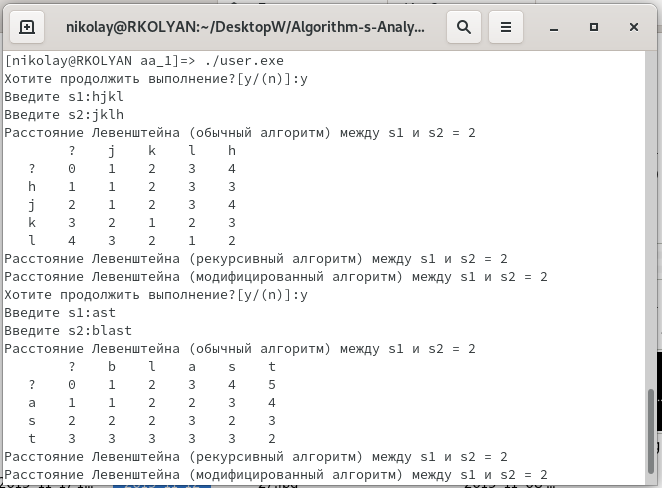
\includegraphics[scale=0.5]{example.png}}
\caption{Пример работы приложения}
\label{images:example}
\end{figure}

\newpage
\subsection{Результаты тестирования}
\begin{table}[h]
\caption{\label{tablice:tests}Результаты тестирования приложения}
\begin{center}
\begin{tabular}{|c|c|c|c|c|}
\hline 
1-я строка & 2-я строка & Результат 1 & Результат 2 & Результат 3 \\ 
\hline 
hjkl & jklh & 2 & 2 & 2 \\ 
\hline 
abcdef & abcfed & 2 & 2 & 2 \\ 
\hline 
astronavt & cosmonavt & 4 & 4 & 4 \\ 
\hline 
baobab & babo & 3 & 3 & 2 \\ 
\hline 
argo & argo & 0 & 0 & 0 \\ 
\hline 
\end{tabular}
\end{center} 
\end{table}

\newpage
\subsection{Постановка эксперимента по замеру времени}
\begin{flushleft}
Для вычисления процессорного времени работы алгоритмов использовалась функция clock(), объявленную в заголовочном файле time.h из библиотеки glibc. \\
Требования к программе, считающей время выполнения алгоритмов:
\begin{itemize}
\item Ввод пользователем таких параметров, как:
\begin{itemize}
\item Максимальная длина для двух строк;
\item Кол-во итераций на каждый рассматриваемый случай (для высчитывания среднего значения);
\end{itemize}
\item Строки должны генерироваться со случайными символами
\item Результаты вычислений должны сохранятся в текстовых файлах
\end{itemize}
\end{flushleft}

\newpage
\subsection{Сравнительный анализ на материале экспериментальных данных}

\begin{figure}[h]
\center{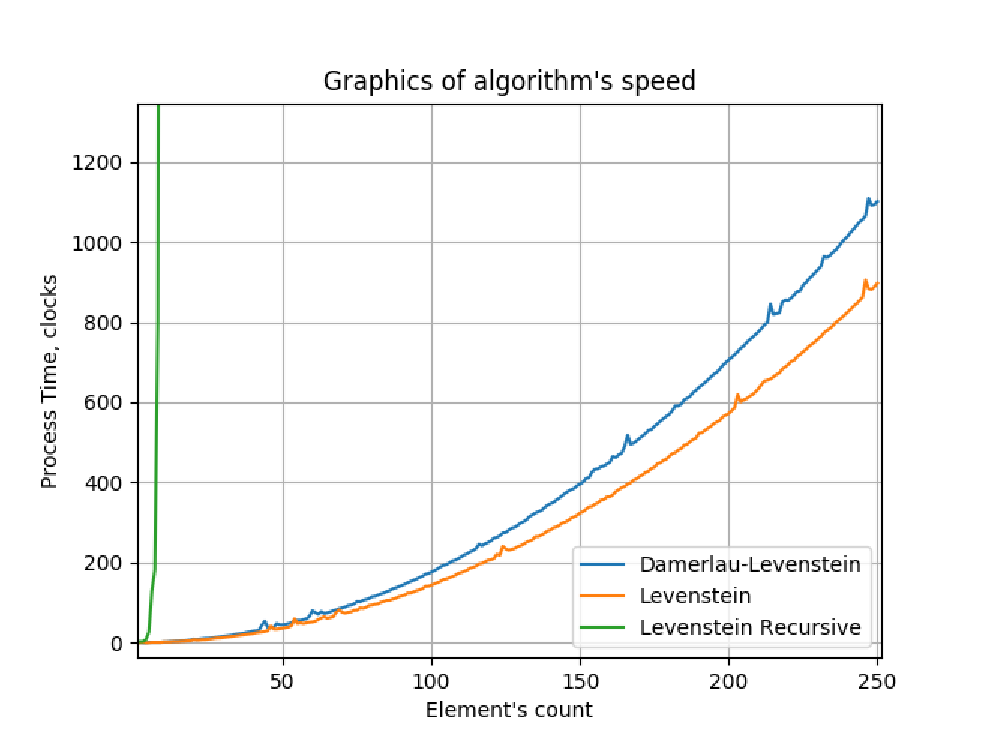
\includegraphics[scale=1]{graphics.eps}}
\caption{График зависимости времени работы алгоритмов от длин строк}
\label{images:graphics}
\end{figure}

Выше приведен график зависимости времени выполнения функций от длины строк. Единица измерения времени – временный такт процессора. \\

Исходя из данного графика можно сделать вывод, что стандартный алгоритм Левенштейна – самый быстрый, а рекурсивный алгоритм – самый медленный. Это может быть обусловлено тем, что в рекурсивной версии алгоритма происходит множество лишних (повторных) вычислений. Возникает дерево рекурсий. \\

\newpage
\subsection{Оценка затрачиваемой памяти}
1)Стандартный алгоритм Левенштейна (\hyperref[listings:listing1]{Листинг Кода 1}): \\
Используемый размер аппаратного стека = 60 байт (включая адрес возврата). \\
Используемый размер динамически выделенной памяти под матрицу: \\
(length1 + 1) * (length2 + 1) * S байт, где \\
length1 – длина первой строки (кол-во символов), \\
length2 – длина второй строки, \\
S – кол-во байт соответствующий выбранному типу данных. \\
Итого: Кол-во всей используемой памяти = 60 + (length1 + 1) * (length2 + 1) * S. \\
\\
2)Рекурсивный алгоритм Левенштейна (\ref{listings:listing2}Листинг Кода 2): \\
Используемый размер аппаратного стека для вызова одной функции = 46 байт, \\
40 байт для конечного вызова. \\
Для того, чтобы рекурсивная функция перестала вызывать саму себя, идет проверка на \\
текущую длину строк. Если хотя бы одна строка имеет текущую длину 1, то находится \\
конечный результат (простейшее редакционное расстояние). \\
И тогда максимальный размер памяти (в аппаратном стеке), используемый во время \\
работы данной функции = (length1 - 1) * (length2 – 1) * 46 + 40 \\
\\
3)Алгоритм Дамерау-Левенштейна (\ref{listings:listing3}Листинг Кода 3): \\
Используемый размер аппаратного стека = 68 байт (включая адрес возврата). \\
Используемый размер динамически выделенной памяти под матрицу: \\
(length1 + 2) * (length2 + 1) * S байт, где \\
length1 – длина первой строки (кол-во символов), \\
length2 – длина второй строки, \\
S – кол-во байт соответствующий выбранному типу данных. \\
Итого: Кол-во всей используемой памяти = 68 + (length1 + 2) * (length2 + 1) * S. \\
В качестве используемого типа данных для матриц был выбран тип integer (4 байт). \\
Тогда сравнивая найденные значения размеров памяти для 1) и 2) получаем выражение: \\
% Вставь сюда формулу сравнения по памяти
Это выражение истинно при значениях \{\{1, 1\}, \{1, 2\}, \{2, 2\}, \{2, 3\}\}, то есть только в этих случаях рекурсивный алгоритм будет эффективнее по памяти, чем стандартный. \\
Сравнивая 2) и 3) получаем: \\
% и сюда тоже
То есть данный случай можно рассматривать как эквивалентный предыдущему. \\